\section{Question 3}\label{sec:q3}    
\subsection{3a}
\textit{Given radiation equilibrium for a laminar boundary layer, derive an expression for the wall temperature. Give explicit formulations for the fluxes involved.}\\
In the case of equilibrium, the radiative heat flux $q_{rad}$ and the conductive heat flux $q_c$ are in balance. So let's first find expressions for these quantities, and then solve for the wall temperature.\\ 
First, the radiative heat flux is defined using:
\begin{equation}\label{eq:qrad}
    q_{rad} = \epsilon \sigma T_{w,eq}^4
\end{equation}
Where $\epsilon$ is the emissivity and $\sigma$ the Boltzmann constant.

Next, the conductive heat flux can be found using:
\begin{equation}\label{eq:qc}
    q_{s} = \alpha (T_{w,ad} - T_w)
\end{equation}
This is where we make our first assumption: We assume that the adiabatic wall temperature is far larger than $T_w$, and furthermore that it can be approximated by:
\begin{equation}
    T_{w,ad} \approx \frac{V_\infty}{2C_{p_\infty}}
\end{equation}
If we combine this with equation \ref{eq:qc}, we now get:
\begin{equation}
    q_c = \alpha \frac{V_\infty}{2c_{p_\infty}}
\end{equation}
Now, we further expand $\alpha$:
\begin{equation}
    \alpha = St \cdot c_p \cdot \rho \cdot V
\end{equation}
So we obtain:
\begin{equation}
    q_c = St c_p \rho V \frac{V_\infty}{2c_{p_\infty}}
\end{equation}

At this point, we can recognise that the question is about an equilibrium situation and we can equate the two fluxes:
\begin{equation}
    \frac{1}{2} St \rho_\infty V_\infty^3  = \epsilon \sigma T_{w,eq}^4
\end{equation}
And solve for $T_{w,eq}$:
\begin{equation}
    T_{w,eq} = \sqrt[4]{\frac{St \rho_\infty V_\infty^3}{2 \epsilon \sigma}}   
\end{equation}

\subsection{3b}
\textit{Starting with the hydrostatic equation, derive the exponential atmosphere
model for the density. State your assumptions.}\\
Start with the hydrostatic equation:
\begin{equation}\label{eq:hydrostatic}
    dp = - \rho g dh
\end{equation}
Assume the atmosphere is made of a perfect gas so we can use the perfect gas law:
\begin{equation}\label{eq:perfectgas}
    p = \rho R T
\end{equation}
Now divide the left side of the hydrostatic equation by the left side of the perfect gas law. Do the same for the right sides, so you get:
\begin{equation}
    \frac{dp}{p} = -\frac{g}{RT} dh
\end{equation}
Now assume two things:
\begin{itemize}
    \item Constant T in the atmosphere.
    \item Ignore variation in the gravitational acceleration: $g = g_0$
\end{itemize}
This enables us to formulate the previous equation as:
\begin{equation}
    \frac{dp}{p} = \frac{d \rho}{\rho} = -\frac{g_0}{RT} dh
\end{equation}
This we can integrate to find an expression for the density as function of altitude:
\begin{equation}
\begin{split}
    \int{\rho_0}{\rho} \frac{d \rho*}{\rho*} = -\frac{g_0}{RT} \int{h_0}{h}dh* \\
    ln\left( \frac{\rho}{\rho_0} \right) = -\frac{g_0}{RT}(h-h_0) \quad with \quad h_0 = 0 \\
    ln\left( \frac{\rho}{\rho_0} \right) = -\frac{g_0}{RT}h \\
    \frac{\rho}{\rho_0} = e^{-\frac{g_0}{RT}h} = e^{-\beta h}\\
\end{split}
\end{equation}
Where parameter $\beta$ is defined as:
\begin{equation}
    \beta = \frac{g_0}{RT}
\end{equation}
Solving for $\rho$ gives us the answer to the question:
\begin{equation}
    \rho = \rho_0 e^{-\frac{g_0}{RT}h} = \rho_0 e^{-\beta h}
\end{equation}

\subsection{3c}
\textit{Provide a clear sketch of a step response, and indicate in this figure the delay
time, td, rise time, tr, peak time, tp, maximum percentage overshoot, Mp, and settling
time, ts}\\
\begin{figure}[H]
    \centering
    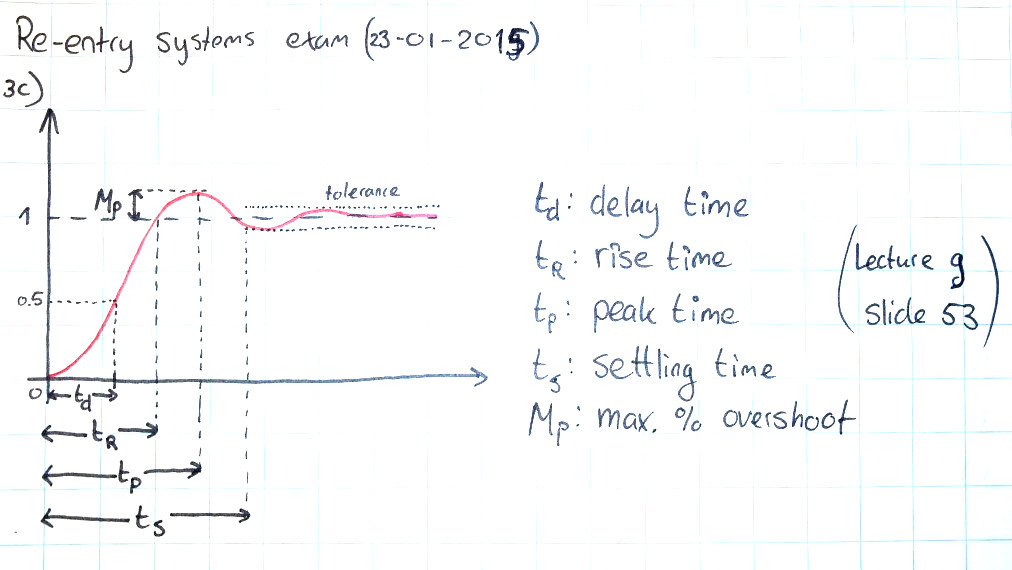
\includegraphics[width=0.9\columnwidth]{Figures/picture_step.jpg}
    \caption{A beautiful Renaissance painting with the features of a step function}
    \label{fig:step}
\end{figure}

\subsection{3d}
\textit{Provide a clear drawing of a parachute/payload system and indicate the
following elements: cover, deployment bag, pilot chute, bridle, canopy, main parachute,
suspension lines, riser, payload.}\\
\begin{figure}[H]
    \centering
    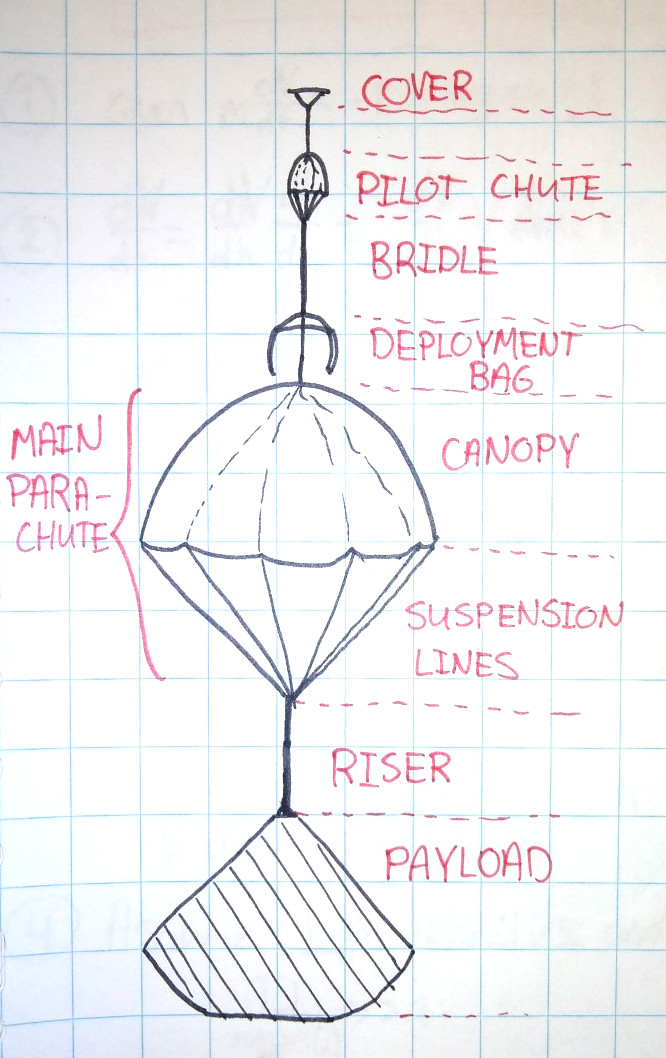
\includegraphics[width=0.4\columnwidth]{Figures/picture_parachutes.jpg}
    \caption{The anatomy of a parachute}
    \label{fig:chute}
\end{figure}